\section{Trivial Example}
Looking back at \cref{fig:running-example}, this example was created by human hands. In its design there is an attempt to maximize throughput by using parallel execution and creating different branches for different types of items. Yet how would a computer, given the same set of modules and the same set of items to produce, be able to arrive to such a configuration?

To kick off this discussion, we will provide a trivial example of how this factory could be constructed. Let us say that we are given the same modules as in \cref{fig:running-example}. In addition we are supposed to produce three types of items, a doll, a rocking horse and a wooden sword as described in \cref{fig:toy-recipes}. Obviously these items can be produced by the running example. The same is true for the trivial configuration shown in \cref{fig:trivial-example}.  

\begin{figure}[h]
\centering
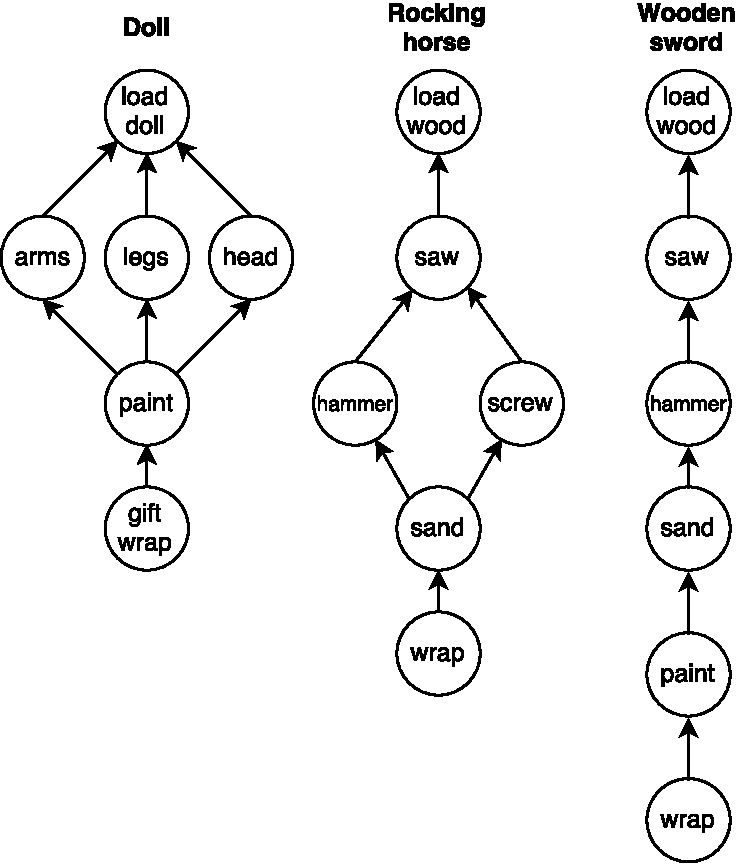
\includegraphics[width=\textwidth]{toyrecipes.pdf}
\caption{Acyclic dependency graphs describing three item types. From left to right, doll, rocking horse and wooden sword.}
\label{fig:toy-recipes}
\end{figure}

This trivial configuration is obviously a poorer choice. In the old configuration no item had to pass through a module, where it was not worked upon. At least when excluding the transport module. We originally got around this issue by producing items on separate branches. In comparison, the trivial configuration is made of a single line.

In addition the trivial example uses the minimal amount of modules needed to process our orders. This means that we see no parallel execution of any items as in the previous execution. 

Yet, the advantage of the trivial example is that it is very simple to generate using a computer. This can not be said for the man made configuration. To produce this trivial example we have to compose the three graphs in \cref{fig:toy-recipes}. On the resulting dependency graph we then perform a topological sort. This gives us an ordered list of work types, which we can then use as a blueprint to place down modules in a line, connecting them from left to right.

A dependency graph may of course have several topological sorts. Because of this we could just generate a configuration for each of these sorts. Each of these candidate solutions can then be set up in our UPPAAL model, and we can find the execution time of their fastest trace. The configuration with the fastest trace is then deemed the best fitting candidate.  Yet, again this configuration would most likely still be poor compared to the one we created ourselves.

Because of this we want ways in which we from a trivial configuration are able to branch out production when needed. We also want to allow for some kind of parallel execution.  In the following section we will formally describe, how we may transform lines of modules so that our configurations gains these qualities.


\begin{figure}[h]
\centering
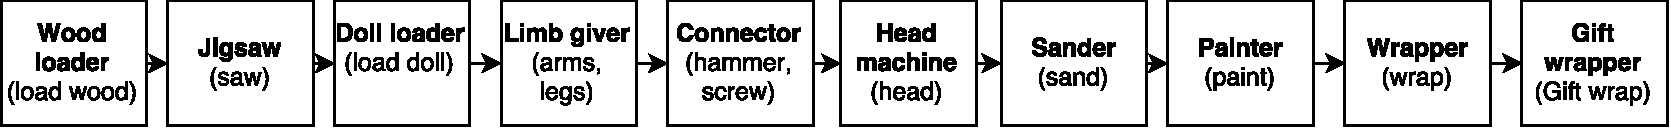
\includegraphics[width=\textwidth]{trivialexample.pdf}
\caption{A trivial configuration of a toy factory layout}
\label{fig:trivial-example}
\end{figure}





